\chapauthor{Садовский М.Е.\\Жмырко А.В.}
\chapter{Методика и средства компонентного проектирования интерфейсов ostis-систем}
\chapauthortoc{Садовский М.Е.\\Жмырко А.В.}
\label{chapter_ui_design}

\vspace{-7\baselineskip}
\begin{SCn}
\begin{scnrelfromlist}{автор}
	\scnitem{Садовский М.Е.}
	\scnitem{Жмырко А.В.}
\end{scnrelfromlist}
\bigskip
	
\scntext{аннотация}{Проектирование интерфейса – это один из наиболее важных  этапов разработки любой системы.
Пользователь при обращении с интерфейсом должен представить себе, какая информация о выполняемой задаче у него существует, и в каком состоянии находятся средства, с помощью которых он будет решать данную задачу. Эффективность работы пользователя и его интерес обеспечивает правильно сформулированная методика разработки и проектирования пользовательского интерфейса. \newline
В настоящее время организация взаимодействия пользователя с компьютерной системой лежит парадигма \textbf{грамотного пользователя},	который знает, как управлять системой и несёт полную ответственность за качество взаимодействия с ней.
Многообразие форм и видов интерфейсов приводит к необходимости пользователя  адаптироваться к каждой конкретной системе, обучаться принципам взаимодействия с ней для решения необходимых ему задач. \newline
Проектирование пользовательских интерфейсов включает в себя ряд последовательных этапов.
В рамках главы будут рассмотрены этапы проектирования традиционных пользовательских интерфейсов и этапы проектирования адаптивных интеллектуальных мультимодальных пользовательских интерфейсов.}
\end{SCn}

\section{Действия и методики проектирования интерфейсов ostis-систем}

Среди существующих методик проектирования адаптивных интеллектуальных мультимодальных пользовательских интерфейсов можно выделить методики,
предложенные в \scncite{Ehlert2003} и  \scncite{Kong2011}.

В рамках работы \scncite{Ehlert2003} выделяется 4 основных этапа проектирования:
\begin{textitemize}
    \item анализ;
    \item разработка интерфейса;
    \item оценка интерфейса;
    \item доработка и усовершенствование.
\end{textitemize}

Этап анализа является, вероятно, самой важной фазой в любом процессе проектирования, но тем более в проектировании интерфейсов ostis-систем. В
процессе проектирования обычного неинтеллектуального интерфейса
необходимо проанализировать, кто является обычным пользователем, какие задачи интерфейс должен поддерживать. 

В пользовательском интерфейсе часто нет среднего пользователя.
В идеале, пользовательский интерфейс должен быть способен адаптироваться к любому пользователю в любой среде. Поэтому используемая техника адаптации должна быть разработана таким образом, чтобы она могла поддерживать все типы пользователей.

Этап \textit{анализа} включает выполнение четырех взаимосвязанных видов анализа:
\begin{textitemize}
    \item функциональный анализ;
    \item анализ данных;
    \item анализ пользователей;
    \item анализ среды.
\end{textitemize}

В рамках \textit{функционального анализа} необходимо дать ответ на вопрос: "каковы \uline{основные функции системы}?".
В рамках \textit{анализа данных} необходимо определить \uline{значение и структуру данных}, используемых в приложении.
В рамках \textit{анализа пользователей} необходимо выделить \uline{типы пользователей и их возможности} в интеллектуальном
и когнитивном плане.
В рамках \textit{анализа среды} необходимо определить \uline{требования, предъявляемые к среде}, в которой будет работать система.

Результатом данного этапа является \uline{cпецификация целей и информационных потребностей пользователя}, а также
\uline{спецификация функций и информации}, которые требуются системе.

\textit{Разработка интерфейса} включает следующие шаги:
\begin{textitemize}
	\item \textit{создание модели интерфейса} в соответствии с этапом анализа;
	\item реализация модели интерфейса.
\end{textitemize}

Результатом данного этапа является \uline{пользовательский интерфейс}, который, по мнению разработчика, удовлетворяет требованиям пользователей и соответствует требованиям, сформулированным на этапе анализа.

\textit{Оценка интерфейса} предполагает, что:
\begin{textitemize}
	\item требования, которые были сформулированы на этапе анализа, должны быть удовлетворены;
	\item эффективность модели интерфейса должна быть исследована.
\end{textitemize}

На этапе \textit{оценки интерфейса} необходимо вернуться к требованиям \textit{этапа анализа}. Требования, которые
были сформулированы на \textit{этапе анализа}, должны быть выполнены, а также должна быть исследована эффективность модели интерфейса.
Чтобы определить эту эффективность, необходимо определить критерии эффективности.

Очень важным, но субъективным критерием является удовлетворенность пользователя. Поскольку пользователь должен работать с интерфейсом, он имеет право голоса в вопросе о том, удобно ли работать с интерфейсом и т.п.

Критериями эффективности могут выступать различные показатели, такие как:
\begin{textitemize}
	\item количество ошибок;
	\item время выполнения задачи;
	\item отношение пользователя к интерфейсу;
	\item т.д.
\end{textitemize}

\textit{Доработка и усовершенствование} осуществляется на основе проблем, выявленых на этапе оценки. В рамках данного этапа вносится ряд улучшений в модель интерфейса. Затем начинается новый цикл проектирования. Этот итеративный процесс будет продолжаться до тех пор, пока результат оценки не будет удовлетворять обозначенным требованиям. 

Методика, предложенная в \scncite{Kong2011} включает 6 этапов:
\begin{textitemize}
	\item моделирование пользовательского интерфейса (описание абстрактного пользовательского интерфейса);
	\item проектирование пользовательского интерфейса по умолчанию (стандартная версия, конкретный пользовательский интерфейс);
	\item разработка пользовательского интерфейса (расширение или замена пользовательского интерфейса по умолчанию) - этот шаг опускается, когда система генерирует пользовательский интерфейс по умолчанию автоматически;
	\item создание контекста использования (идентификация и создание контекста использования - модели пользователя, модель устройства и модель среды/платформы);
	\item адаптация пользовательского интерфейса - автоматически - (адаптация пользовательского интерфейса во время выполнения для соответствия конкретного контекста использования);
	\item кастомизация пользовательского интерфейса - настройка пользовательского интерфейса самим пользователем (адаптируемость).
\end{textitemize}

На основе рассмотренных методик проектирования интерфейсов можно выделить следующие общие этапы:
\begin{textitemize}
\item анализ контекста использования и задач пользователей;
\item проектирование и разработка интерфейса;
\item оценка качества спроектированного интерфейса.
\end{textitemize}

Среди недостатков предложенных подходов можно выделить:
\begin{textitemize}
	\item знания по каждому этапу проектирования находятся у разных специалистов в неформализорованном неунифицированном виде;
	\item отсутствие этапа формализованного документирования этапов проектирования приводит в дальнейшем в необходимости создания отдельных help-систем для пользователей, разработчиков и т.д.
\end{textitemize}

Предлагается использовать онтологический подход на основе семантической модели в процессе проектирования и реализации адаптивного интеллектуального мультимодального пользовательского интерфейса. Такой интерфейс предлагается рассматривать как специ-
ализированную подсистему для решения интерфейсных задач пользователя, состоящую из базы знаний и решателя интерфейсных задач. 

Описание модели базы знаний и решателя предлагается осуществлять на основе универсального унифицированного языка представления знаний, что обеспечит совместимость между этими компонентами.

Архитектура интерфейса такой системы была рассмотрена на рисунке "Архитектура интеллектуального интерфейса"{}.

\scnheader{Архитектура интеллектуального интерфейса}
\begin{figure}[h]
	\centering
	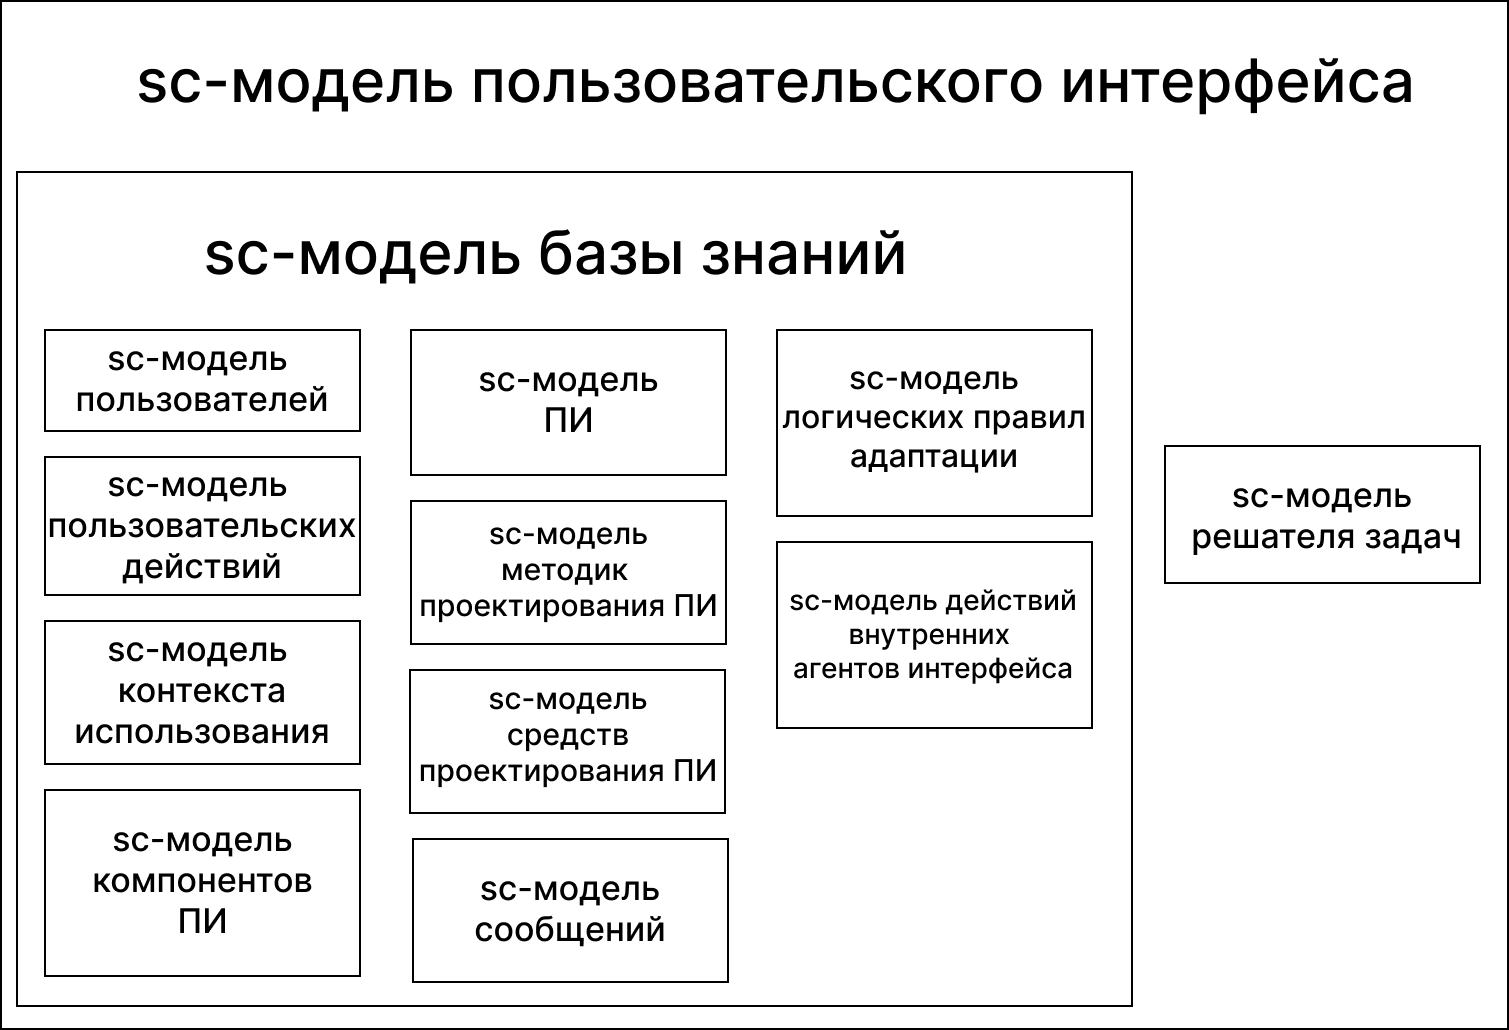
\includegraphics[scale=0.15]{images/part5/sc-model-ui.png}
\end{figure}

Таким образом, предлагаемая методика проектирования интерфейсов ostis-систем будет включать:
\begin{textitemize}
\item анализ пользователя, его задач и целей, а также контекста использования;
\item анализ требований к пользовательскому интерфейсу;
\item проектирование пользовательского интерфейса по умолчанию;
\item разработка пользовательского интерфейса;
\item анализ пользовательского интерфейса и его адаптации.
\end{textitemize}

Поскольку знания о конкретном этапе обычно находятся у разных экспертов, особенностью предлагаемого подхода является обязательное формализованное документирование знаний в унифицированном виде и применение на каждом из этапов компонентного подхода.

Для применения компонентного подхода предлагается использовать \textit{библиотеку многократно используемых компонентов} базы знаний, решателя задач и интерфейса.

\scnheader{Анализ пользователя, его задач и целей, а также контекста использования}

Результаты первого этапа, такие как: модель конкретного пользователя, его потребности и контекст использования системы (устройство, окружающая среда) должны быть формализованы в рамках соответствующих онтологий базы знаний интерфейса. 
При этом в процессе формализации по необходимости должны быть переиспользованы компоненты базы знаний из библиотеки многократно используемых компонентов, а новые компоненты могут пополнить эту же библиотеку.

\scnheader{Анализ требований к пользовательскому интерфейсу}

Результатом второго этапа являются конечные требования к интерфейсу, которые должны быть сформулированы относительно модели пользователя и его цели, а также относительно контекста использования.

Результаты должны быть также формализованы, а в процессе выполнения могут быть использованы существующие компонент базы знаний из библиотеки многократно используемых компонентов.

\scnheader{Проектирование пользовательского интерфейса по умолчанию}

В соответствии с требованиями к пользовательскому интерфейсу, строится модель адаптивного интеллектуального мультимодального пользовательского интерфейса, которая является результатом третьего этапа.

Такая модель будет включать в себя формализованную модель базы знаний и решателя задач.

При проектировании могут быть использованы компоненты интерфейса, базы знаний и решателя задач. 
Компоненты будут записаны в унифицированном виде, что позволит обеспечить их автоматическую совместимость.

\scnheader{Разработка пользовательского интерфейса}

Результатом четвертого этапа является реализация спроектированного пользовательского интерфейса. В данном случае следует использовать готовые компоненты интерфейса из библиотеки многократно используемых компонентов интерфейса.

\scnheader{Анализ пользовательского интерфейса и его адаптации}
На данном этапе используются готовые компоненты решателя задач.


Таким образом будет сформирована база знаний проектируемого интерфейса, которая автоматически может быть использована в качестве help-системы для пользователей, разработчиков и т.д.



\section{Логико-семантическая модель ostis-системы автоматизации проектирования интерфейсов ostis-систем}
\section{Многократно используемые компоненты интерфейсов ostis-систем}

%\input{author/references}